% !TeX spellcheck = en_GB
\documentclass[answers]{exam}
% addpoints

\ifprintanswers
	\usepackage[type1]{libertine}
	\usepackage[a4paper]{geometry}
	\usepackage{parskip}
\else
\fi

\usepackage{amsmath, amsthm, amssymb} 
\usepackage{tabularx}
\usepackage[english]{babel}
\usepackage{enumitem}
\usepackage{gensymb}
\usepackage{bm}
\usepackage{graphicx}
\usepackage{xcolor}
\usepackage{float}
\usepackage{wrapfig}
\usepackage[makeroom]{cancel}
\usepackage{multicol}
\usepackage{vwcol} 	 % Provides variable multicol
\usepackage{commath} % Provides good differentials
\usepackage{siunitx} % Provides good units
\usepackage{nicefrac}

\usepackage[titletoc,title,toc,page]{appendix}
\usepackage{hyperref}
\hypersetup{
	pdftitle={SJPO Training -- Energy \& Momentum Problem Set},
	pdfauthor={Sun Yudong, Tan Jing Long},
	bookmarksnumbered=true,
	bookmarksopen=true,
	bookmarksopenlevel=2,
	pdfstartview=Fit,
	pdfpagemode=UseOutlines,
	colorlinks=true,
	linkcolor=black,
	filecolor=magenta,      
	urlcolor=blue
}

\newcommand{\uvec}[1]{\boldsymbol{\hat{\textbf{#1}}}}
\def\doubleunderline#1{\underline{\underline{#1}}}

\newenvironment{multicolFigure}
{\par\medskip\noindent\minipage{\linewidth}}
{\endminipage\par\medskip}
% https://tex.stackexchange.com/questions/12262/multicol-and-figures

%\newenvironment{amatrix}[1]{%
%	\left(\begin{array}{@{}*{#1}{c} | c@{}}
%	}{%
%	\end{array}\right)
%}						% https://tex.stackexchange.com/a/2238
%\usepackage{blkarray}	% https://tex.stackexchange.com/a/59519
%\usepackage{mathtools}	% https://tex.stackexchange.com/a/103993

% for comments 			% https://tex.stackexchange.com/a/209668

\begin{document}


\ifprintanswers
	\title{\vspace{-1cm} SJPO Training\\ Energy \& Momentum Problem Set}
	\author{Worked Solutions by Sun Yudong \\ {\small Questions originally compiled by Tan Jing Long on April 23, 2016}}
	\date{April 11, 2018}
\else
	\title{SJPO Training\\ Energy \& Momentum Problem Set}
	\author{Tan Jing Long}
	\date{April 23, 2016}
\fi
\maketitle

\section{General Round}
	\subsection{Collisions}
		\begin{questions}
			\question{A baseball is thrown vertically upward and feels no air resistance. As it is rising,
				\begin{choices}
				\choice{both its momentum and its mechanical energy are conserved.}
				\choice{both its momentum and kinetic energy are conserved.}
				\choice{its kinetic energy is conserved but its momentum is not conserved.}
				\choice{the gravitational potential energy is not conserved but its momentum is conserved.}
				\choice{its momentum is not conserved but its mechanical energy is conserved.}
				\end{choices}
			\begin{solution} E \\Momentum is not conserved because the baseball experiences a net force due to gravity. \end{solution}
			}
		
			\ifprintanswers
				\vfill
			\else
			\fi
			
			\question{A large truck and a small car collided near Bukit Timah road one day and the two vehicles were stuck together. Which vehicle has undergone a larger change in momentum?
				\begin{choices}
				\choice{The car.}
				\choice{The truck.}
				\choice{The momentum change was the same for both vehicles.}
				\choice{One cannot tell which vehicle has undergone a larger momentum change without knowing the final velocity of the combined mass.}
				\choice{One cannot tell which vehicle has undergone a larger momentum change without knowing the masses of the truck and car.}
				\end{choices}
				\begin{solution} C \\By Newton's 3\textsuperscript{rd} Law, the force of the car on the truck is the same as that of the truck on the car. Since $F = \dod{p}{t}$, they undergo the same change in momentum. \end{solution}
			}
			\ifprintanswers
				\pagebreak
			\else
				%\vfill
			\fi
			\question{A fast moving small bullet of mass \(m\) hits and passes through a heavy stationary wooden block of mass \(M\). When the bullet passes through the block,
				\begin{choices}
				\choice{\(M\) and \(m\) experience the same impulse.}
				\choice{The mutual force between the bullet and the wooden block will do the same amount of work.}
				\choice{The bullet's speed will reduce by the same amount as the increase in the wooden block's speed.}
				\choice{The bullet's momentum will reduce by the same amount as the increase in the wooden block's momentum.}
				\choice{The bullet's temperature will increase by the same amount as the increase in the wooden block's temperature.}
				\end{choices}
			\ifprintanswers
				\vfill
			\fi
			\begin{solution} D \\ Total momentum is conserved. Any impulse imparted onto the wooden block must come from the bullet. $M$ and $m$ thus experience the same magnitude of impulse, but the impulse is opposite in direction. \end{solution}
			}
			
			\ifprintanswers
				\vfill
			\else
				\pagebreak
			\fi
			
			\question{Two identical masses are hung on strings of the same length. One mass is released from a height \(H\) above its free-hanging position and strikes the second mass; the two stick together and move off. They rise to height \(h\) given by
			\begin{figure}[h!]
				\begin{center}
					\includegraphics[scale=0.5, clip=false, trim=0 35 0 10]{mcq_2011_10}
				\end{center}
			\end{figure}
			\ifprintanswers
				\vfill
			\fi
			\begin{solutionorbox}[40mm]
				\vspace{-0.5cm}
				\begin{align*}
					\text{GPE} = mgH &= \frac{1}{2}mv_i^2 = \text{KE} \\
					v_i &= \sqrt{2gH} \\
					v_f &= \frac{\cancel{m}v_i}{2\cancel{m}} = \frac{1}{2}\sqrt{2gH}\\
					\text{KE} = \frac{1}{2}(2m)\left(\frac{1}{2}\sqrt{2gH}\right)^2 &= 2mgh = \text{GPE} \\
					\frac{1}{4}\cancel{\left(2mg\right)}H &= \cancel{2mg}h \\
					h = \frac{1}{4}H
				\end{align*}
			\end{solutionorbox}
			}
		
			\ifprintanswers
				\pagebreak
			\else
				\vfill
			\fi
			
			\question{In the diagram shown below, balls \(A\) and \(B\) of mass \(m_A\) and \(m_B\) respectively, hanging on strings of the same length are touching each other when they are at their equilibrium positions. Ball \(A\) is then slightly pulled to the left and released. Which of the following statements are correct after the first collision?
			\begin{figure}[h]
			\begin{center}
			\includegraphics[scale=0.85, clip=false, trim=0 25 0 0]{mcq_2011_9}
			\end{center}
			\end{figure}
				\begin{choices}
				\choice{If \(m_A > m_B\), the next collision will be to the right of the equilibrium position.}
				\choice{If \(m_A < m_B\), the next collision will be to the right of the equilibrium position.}
				\choice{The next collision will be at the equilibrium position.}
				\choice{There is not enough information in the question to predict any of the above outcomes.}
				\end{choices}
			
			\ifprintanswers
				\vspace{1cm}
			\fi
			
			\begin{solution} C \\ After collision, we have 2 pendulums of the same length. Since the period of a pendulum, given by \[T = 2\pi\sqrt{\frac{l}{g}}~,\] is independent of mass, we know that their quarter-period will coincide regardless of their masses. Thus, they will meet again at the same point (i.e. the equilibrium point). \par For now, just take that this expression for the period of a pendulum is true and correct. We will derive it when we eventually get to the chapter of Oscillation. \par The derivation itself is not complicated. If you are feeling up to it, do look up ``Simple Harmonic Motion" for hints on how to do it. \end{solution}
			% For the derivation of the period of a pendulum, refer to Appendix \ref{appdx:pendulum}. Note that the derivation involves concepts that we have yet to learn in class.
			}
			
			\ifprintanswers
				\pagebreak
			\else
				\vfill
			\fi
			
			\question{A soccer ball approaches a player at \(v=\SI{12}{\meter/\second}\). At what velocity \(v\) should the player's foot move in order to stop the ball upon contact? Assume that the mass of the foot is much greater than that of the ball and that the collision is elastic.
				\begin{choices}
				\choice{\(u=\SI{12}{\meter/\second}\) in the direction opposite to the original velocity of the ball.}
				\choice{\(u=\SI{6}{\meter/\second}\) in the direction opposite to the original velocity of the ball.}
				\choice{\(u=\SI{6}{\meter/\second}\) in the same direction as the original velocity of the ball.}
				\choice{\(u=\SI{0}{\meter/\second}\), i.e. he should hold his foot very still.}
				\choice{This feat cannot be done.}
				\end{choices}
			\ifprintanswers
				\vfill
			\fi
			\begin{solution} C \\
				We first write down the conservation of momentum and kinetic energy:
				\begin{align*}
					m_{\! f}u_{\! f} + m_bu_b &= m_{\! f}v_{\! f} + m_bv_b \\
					\frac{1}{2}m_{\! f}u_{\! f}^2 + \frac{1}{2}m_bu_b^2 &= \frac{1}{2}m_{\! f}v_{\! f}^2 + \frac{1}{2}m_bv_b^2
				\end{align*}
				Simplifying:
				\begin{align}
					m_{\! f}u_{\! f} + m_bu_b &= m_{\! f}v_{\! f}  &\implies m_bu_b &= m_{\! f}\left(v_{\! f}-u_{\! f}\right) \label{eqn:6:com}\\
					m_{\! f}u_{\! f}^2 + m_bu_b^2 &= m_{\! f}v_{\! f}^2 &\implies m_bu_b^2 &= m_{\! f}\left(v_{\! f}^2-u_{\! f}^2\right) \label{eqn:6:coe}
				\end{align}
				Dividing \eqref{eqn:6:coe} with \eqref{eqn:6:com}, we obtain the classic equation of the relative speeds of approach and separation:
				\begin{align}
					u_b = v_{\! f} + u_{\! f} \label{eqn:6:rsoa}
				\end{align}
				At this point, as the mass of the feet is much greater than the mass of the mass of the ball, we can safely take that any momentum/energy imparted onto the feet by the ball is negligible, and thus $v_{\! f} = u_{\! f}$, obtaining $u_{\! f} = \nicefrac{12}{2} = \SI{6}{\meter\per\second}$ in the same direction as the original velocity $u_b$ of the ball.
				
				We can of course substitute \eqref{eqn:6:rsoa} into \eqref{eqn:6:com}:
				\begin{align*}
					m_bu_b &= m_{\! f}\left[\left(u_b - u_{\! f}\right) -u_{\! f}\right] \\
					&= m_{\! f} \left[u_b - 2u_{\! f}\right] \\
					2m_{\! f}u_{\! f} &= u_b\left(m_{\! f}-m_b\right) \\
					u_{\! f} &= \frac{1}{2} u_b \left[\frac{m_{\! f} - m_b}{m_{\! f}}\right]
				\end{align*}
				Indeed, if $m_{\! f} \gg m_b~$, then $~\displaystyle \frac{m_{\! f} - m_b}{m_{\! f}} \to 1$ and $\displaystyle u_{\! f} \to \frac{1}{2}u_b = \SI{6}{\meter\per\second}$
				
				{\color{black!70!} Interestingly, if $m_{\! f} = 2m_b$, then $u_{\! f} = 3$ and $v_{\! f} = 9$. Your feet will fly backwards at \SI{9}{\meter/\second} or \SI{32.4}{\kilo\meter/\hour} ... ouch}
				
			\end{solution}
			}
			
			\ifprintanswers
			\else
				\pagebreak
			\fi
			
			\question{Suppose \(\SI{1.0}{\kilo\gram}\) of clay travelling at speed \(v\) smashes into \(\SI{1.0}{\kilo\gram}\) of clay which is not moving. They stick and become one \(\SI{2.0}{\kilo\gram}\) lump of clay. What proportion of the kinetic energy in the originally moving lump was turned into heat and sound during the collision?
				\begin{choices}
				\choice{0\%}
				\choice{25\%}
				\choice{50\%}
				\choice{75\%}
				\choice{100\%}
				\end{choices}
			\begin{solution} C \\
				First, we use the conservation of momentum to find the final velocity $v_{\! f}$
				\begin{equation*}
					v_{\! f} = \frac{\cancel{m}v}{2\cancel{m}} = \frac{1}{2} v
				\end{equation*}
				Then we find the initial and final kinetic energy:
				\begin{align*}
					\text{KE}_i = \frac{1}{2}mv^2 && \text{KE}_{\! f} &= \frac{1}{2}(2m)\left[\frac{1}{2} v\right]^2 \\
					&&& = \frac{1}{2}m\left[\frac{1}{2}\right]v^2
				\end{align*}
				Thus, 
				\begin{equation*}
					\frac{\text{KE}_i - \text{KE}_{\! f}}{\text{KE}_i} = \frac{1}{2} \implies 50\%
				\end{equation*}
				It is naturally much faster by observation after finding the initial and final KE.
			\end{solution}
			}
			
			\question{A \(\SI{8.0}{\gram}\) bullet is shot into a \(\SI{4.0}{\kilogram}\) block, at rest on a frictionless horizontal surface. The bullet remains lodged in the block. The block moves toward a spring and compresses it by \(\SI{9.4}{\centi\meter}\). The force constant of the spring is \(\SI{1000}{\newton/\meter}\). Determine the initial speed of the bullet.
			\begin{solutionorbox}[40mm] \(\SI{740}{\meter/\second}\) \\
				Right after the collision, the block and the bullet is moving at:
				\begin{equation*}
					v_c = \frac{m_{\text{bullet}}v_{\text{bullet}}}{m_{\text{bullet}} + m_{\text{block}}}
				\end{equation*}
				and the combined block and bullet has kinetic energy:
				\begin{align*}
					\text{KE} &= \frac{1}{2}\left[m_{\text{bullet}} + m_{\text{block}}\right]v_c^2 \\
					&= \frac{1}{2}\left[m_{\text{bullet}} + m_{\text{block}}\right]\left[\frac{m_{\text{bullet}}v_{\text{bullet}}}{m_{\text{bullet}} + m_{\text{block}}}\right]^2 \\
					&= \frac{1}{2}\left[\frac{m_{\text{bullet}}^2v_{\text{bullet}}^2}{m_{\text{bullet}} + m_{\text{block}}}\right]
				\end{align*}
				All the KE is converted into EPE:
				\begin{align*}
					\text{EPE} = \cancel{\frac{1}{2}}kx^2 &= \cancel{\frac{1}{2}}\left[\frac{m_{\text{bullet}}^2v_{\text{bullet}}^2}{m_{\text{bullet}} + m_{\text{block}}}\right] = \text{KE} \\
					\frac{kx^2\left[m_{\text{bullet}} + m_{\text{block}}\right]}{m_{\text{bullet}}^2} &= v_{\text{bullet}}^2 \\
					v_{\text{bullet}} &= \sqrt{\frac{kx^2\left[m_{\text{bullet}} + m_{\text{block}}\right]}{m_{\text{bullet}}^2}} \\
					&= \SI{740}{\meter\per\second} &\text{(2 s.f.)}
				\end{align*}
			\end{solutionorbox}
			}
			
			\question{A man of mass \(m\) on an initially stationary boat gets off the boat by leaping to the left in an exactly horizontal direction. Immediately after the leap, the boat, of mass \(M\), is observed (by an Earth obsever) to be moving to the right at speed \(v\). How much work did the man do during the leap (both to his own body and on the boat)?
			\begin{solutionorbox}[40mm] \[\frac{1}{2}\left(M+\frac{M^2}{m}\right)v^2\] 
				We first find the velocity of the man:
				\begin{equation*}
					v_m = \frac{Mv}{m}
				\end{equation*}
				Work done by the man becomes the kinetic energy of the boat and the man:
				\begin{align*}
					W &= \text{KE}_{b} + \text{KE}_{m} \\
					&= \frac{1}{2}Mv^2 + \frac{1}{2}m\left(\frac{Mv}{m}\right)^2 \\
					&= \frac{1}{2}\left(M+\frac{M^2}{m}\right)v^2
				\end{align*}
			\end{solutionorbox}
			}
			
			
			%\question{A ball of mass \(\SI{0.25}{\kilogram}\) is thrown with a speed of \(\SI{30}{\meter/\second}\). The ball strikes a bat and it is hit straight back along the same line at a speed \(\SI{50}{\meter/\second}\). The variation of the interaction force when the ball is in contact with the bat is shown as an isosceles triangle in the figure below. Determine the maximum force exerted by the bat on the ball. \begin{figure}[h] \begin{center} \includegraphics[scale=0.62, clip=false, trim=0 45 0 30]{mcq_2010_31} \end{center} \end{figure} \begin{solutionorbox}[45mm] \(\SI{5000}{\newton}\) \end{solutionorbox} }
			
			%\question{Consider two carts, \(A\) and \(B\), of masses \(m\) and \(2m\) respectively, are initially at rest on an air track. If you push both carts with the same force and for the same duration of time, the ratio of final momentum of cart \(A\) to final momentum of cart \(B\) is 	\begin{choices} 	\choice{1 : 4} 	\choice{1 : 2} 	\choice{1 : 1} 	\choice{2 : 1} 	\choice{4 : 1} 	\end{choices} \begin{solution} C \end{solution} }
			
			\pagebreak
			\question{A body at rest explodes breaking into three pieces which move off at different velocities, all in the same horizontal plane. The following figure shows the experimental results as drawn from a stroboscopic photograph of the event. The time interval between flashes was \(\SI{0.10}{\second}\). The pieces \(X\) and \(Y\) travel at right angles to each other and are collected after the explosion and their masses are found to be \(\SI{2.0}{\kilo\gram}\) and \(\SI{1.0}{\kilo\gram}\) respectively. Piece \(Z\) was unfortunately lost after the explosion. What is the mass of piece \(Z\)?
			\begin{figure}[h]
			\begin{center}
				\ifprintanswers
					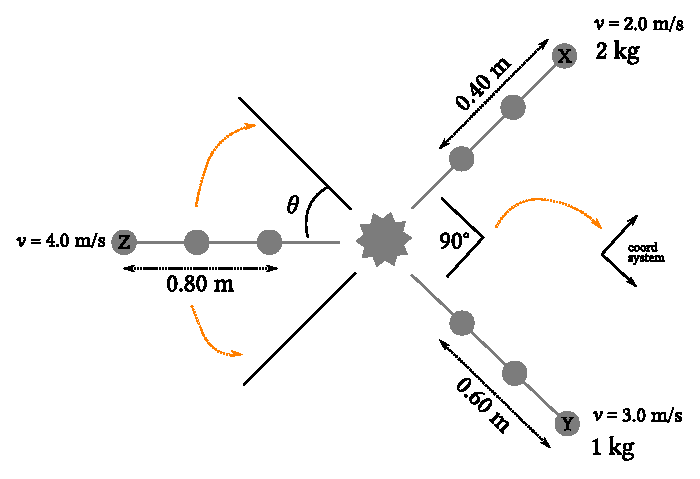
\includegraphics[width=0.7\textwidth]{mcq_2014_23.eps}
					\vspace{-1cm}
				\else
					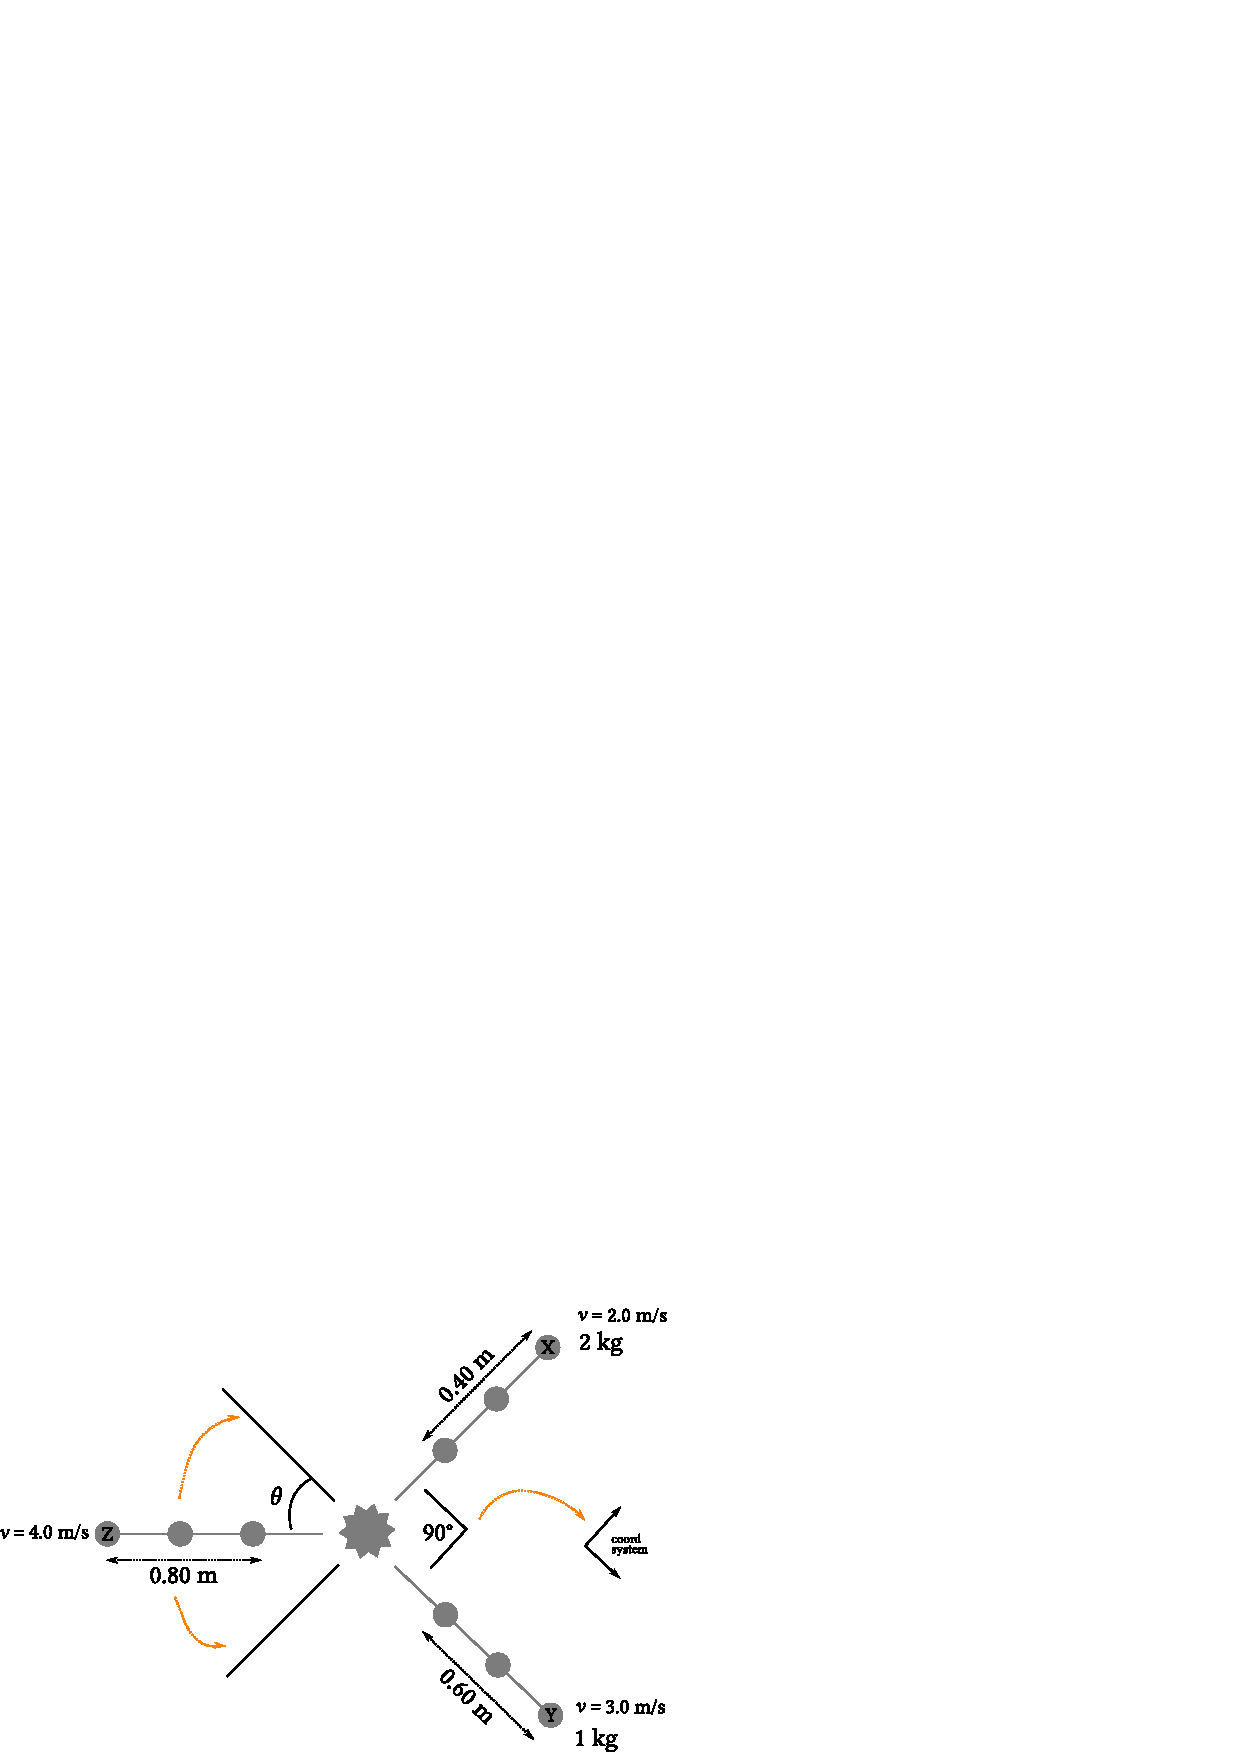
\includegraphics[scale=0.43, clip=false, trim=0 0 0 0]{mcq_2014_23.PNG}
				\fi
			\end{center}
			\end{figure}
				\begin{choices}
				\choice{\(\SI{1.25}{\kilogram}\)}
				\choice{\(\SI{1.50}{\kilogram}\)}
				\choice{\(\SI{2.00}{\kilogram}\)}
				\choice{\(\SI{0.85}{\kilogram}\)}
				\choice{\(\SI{3.00}{\kilogram}\)}
				\end{choices}
			\begin{solution} A \\
			Since $X$ and $Y$ are at right angles to each other, we can resolve all momentum using the directions of $X$ and $Y$ as our coordinate system. Applying the conservation of momentum:
			\begin{align}
				m_zv_z \sin \theta &= m_xv_x \label{eqn:10:1}\\
				m_zv_z \cos \theta &= m_yv_y \label{eqn:10:2}
			\end{align}
			Dividing \eqref{eqn:10:1} by \eqref{eqn:10:2}:
			\begin{equation}
				\tan \theta = \frac{m_xv_x}{m_yv_y} = \frac{4}{3} \label{eqn:10:theta}
			\end{equation}
			Substituting \eqref{eqn:10:theta} back into \eqref{eqn:10:1}:
			\begin{align*}
				m_z &= \frac{m_xv_x}{v_z \sin\theta} \\
				&= \frac{4}{4\left(\frac{4}{5}\right)} \\
				&= \SI{1.25}{\kilogram}
			\end{align*}
			\end{solution}
			}
		
		\end{questions}
	\pagebreak
	\subsection{Work, Energy and Power}	
		\begin{questions}
			\question{Two equal masses are raised at constant velocity by ropes that run over pulleys as shown. Mass \(B\) is raised twice as fast as mass \(A\). The magnitudes of the forces are \(F_A\) and \(F_B\), while the power supplied respectively \(P_A\) and \(P_B\). Which of the following statement(s) is correct?
			\begin{figure}[h]
			\begin{center}
			\includegraphics[scale=0.9, clip=true, trim=0 14 0 13]{mcq_2009_6}
			\end{center}
			\end{figure}
				\begin{choices}
				\choice{\(F_B=F_A\), \(P_B=P_A\).}
				\choice{\(F_B=F_A\), \(P_B=2P_A\).}
				\choice{\(F_B=2F_A\), \(P_B=P_A\).}
				\choice{\(F_B=2F_A\), \(P_B=2P_A\).}
				\choice{\(F_B=2F_A\), \(P_B=4P_A\).}
				\end{choices}
				\begin{solution} B \\ Since they are moving at constant velocity, the $F_A = F_B = mg$. Since $P = Fv$, and Mass $B$ is raised twice as fast, $P_B=2P_A$\end{solution}
			}
		
			\ifprintanswers
				\vfill
			\fi
			\question{A tennis ball bounces on the floor three times. If each time it loses 23.0\% of its energy due to heating, how high does it bounce after the third time, given that we released it \(\SI{4.90}{\meter}\) from the floor?
			\begin{solutionorbox}[40mm] 
				\begin{equation*}
					h \propto E \implies h = (0.77)^3(4.90) = \SI{2.24}{\meter}
				\end{equation*}
			\end{solutionorbox}
			}
			\ifprintanswers
			\vfill
			\fi
			
			\pagebreak
			
			\question{A \(\SI{50}{\kilo\gram}\) person stands on a \(\SI{25}{\kilo\gram}\) platform. He pulls on the rope that is attached to the platform via the frictionless pulley system shown here. If he pulls the platform up at a steady rate, with how much work does the person do in order to pull the platform (and himself) up by \(\SI{2.0}{\meter}\)? Ignore friction.
			\begin{figure}[h]
			\begin{center}
			\includegraphics[scale=0.5, clip=false, trim=0 0 0 0]{mcq_2014_5}
			\end{center}
			\end{figure}
		
				\begin{choices}
				\choice{\(\SI{1000}{\joule}\)}
				\choice{\(\SI{750}{\joule}\)}
				\choice{\(\SI{630}{\joule}\)}
				\choice{\(\SI{500}{\joule}\)}
				\choice{\(\SI{1500}{\joule}\)}
				\end{choices}
			\begin{solution} E 
				\begin{equation*}
					W = \Delta \text{GPE} = mgh = (50 + 25)(9.81)(2.0) = 1500 \text{ (2 s.f.)}
				\end{equation*}
			\end{solution}
			}
		
			\ifprintanswers
				\pagebreak
			\fi
			
			\question{The same constant force is used to accelerate two carts of the same mass on frictionless tracks. The force applied to cart \(A\) is twice as long in time as it is applied to cart \(B\). The work the force does on \(A\) is \(W_A\); that on \(B\) is \(W_B\). Which statement is correct?
				\begin{choices}
				\choice{\(W_A=W_B\).}
				\choice{\(W_A=\sqrt{2}W_B\).}
				\choice{\(W_A=2W_B\).}
				\choice{\(W_A=4W_B\).}
				\choice{\(W_B=2W_A\).}
				\end{choices}
				\begin{solution} D
				\begin{align*}
					W &= F \cdot S = F \cdot \left(at^2\right) \implies W \propto t^2 \\
					&\implies \frac{W_A}{W_B} = 2^2 = 4 \implies W_A = 4W_B
				\end{align*}
				\end{solution}
			}
			
			%\question{A block of mass \(m\) is hung from a light vertical spring of spring constant \(k\), which is hung in turn from another identical spring. The amount by which each spring stretches is \(x\). Determine the total elastic potential energy of the system when at rest. \begin{solutionorbox}[60mm] \(mgx\) \end{solutionorbox} }
			
			\ifprintanswers
				\vfill
			\fi
			
			\question{A car with mass \(\SI{100}{\tonne}\) starts from rest, driven by an engine with uniform power output of \(\SI{5}{\mega\watt}\). Forty seconds later, it is \(\SI{400}{\meter}\) from the starting point and has velocity \(v\). If the resistance experienced by the car is always 0.1 times of the car weight, what is the value of \(v\)? Take \(g\) to be \(\SI{10}{\meter/\second^2}\).
			\begin{solutionorbox}[40mm] \(\SI{57}{\meter/\second}\)
			\begin{multicols}{2}
				\noindent 
				\begin{align*}
					W_{\text{engine}} &= P \times t \\
					&= \left(5 \times 10^6\right)\left(40\right) \\
					&= 2.0 \times 10^8
				\end{align*}
				\begin{align*}
					W_{\text{resistive}} &= F \cdot s \\
					&= 0.1mg \cdot s \\
					&= \left(0.1 \times 100 \times 10^3 \times 10 \right)\left(400\right) \\
					&= 4.0 \times 10^7
				\end{align*}
			\end{multicols}
			\noindent
			\vspace{-1cm}
			\begin{align*}
				\text{KE} = \sum W &= W_{\text{engine}} - W_{\text{resistive}} \\
				\frac{1}{2} m v^2 &= 2.0 \times 10^8 - 4.0 \times 10^7 \\
				v &= \sqrt{\frac{2\times 1.6 \times 10^8}{100 \times 10^3}} \\
				&= \SI{57}{\meter/\second} &\text{(2 s.f.)}
			\end{align*}
			\end{solutionorbox}
			}
		
			\ifprintanswers
				\vfill
			\fi
			
			%\question{Two springs, \(S_1\) and \(S_2\), have negligible masses and the spring constant of \(S_1\) is 1/3 that of \(S_2\). When a block is hung from the springs as shown below and the springs come to equilibrium again, what is the ratio of the work done in stretching \(S_1\) to the work done in stretching \(S_2\)? \begin{figure}[h] \begin{center} \includegraphics[scale=0.75, clip=false, trim=0 25 0 10]{mcq_2011_12} \end{center} \end{figure} \begin{solutionorbox}[55mm] 3 \end{solutionorbox} }
			
			\pagebreak
			
			\question{A \(\SI{2}{\kilogram}\) mass slides across a rough surface and its kinetic energy is plotted as a function of distance. What is the time that it took to slide across the surface?
			\begin{figure}[h]
			\begin{center}
			\includegraphics[scale=0.42, clip=false, trim=0 60 0 10]{mcq_2012_20}
			\end{center}
			\end{figure}
			\begin{solutionorbox}[70mm] \(2\sqrt{2}~\SI{}{\second}\)
				\begin{multicols}{2}
					\noindent
					\begin{align*}
					W = \Delta E_k &= F \cdot s \\
					F &= \frac{50}{10} = 5 \\
					\implies a &= \frac{F}{m} = \frac{5}{2} \\
					\end{align*}
					\begin{align*}
					v_i &= \sqrt{\frac{E_k}{\frac{1}{2} m}} \\
					&= \sqrt{\frac{50}{\frac{1}{2} \cdot 2}} \\
					&= \sqrt{50} = 5\sqrt{2}
					\end{align*}
				\end{multicols}
				\vspace{-0.7cm}
				\begin{equation*}
					t = \frac{v_i - 0}{a} = \frac{5\sqrt{2}}{\nicefrac{5}{2}} = 2\sqrt{2} ~\SI{}{\second}
				\end{equation*}
				
			\end{solutionorbox}
			}
		
			\ifprintanswers
			\vfill
			\fi
			
			%\pagebreak
			\question{The magnitude of the resistive force on a cruising plane is directly proportional to \(v^2\) where \(v\) is the plane's velocity. If the power expended by the plane is \(P\) when the plane is cruising at velocity \(v\), what will be the power expended by the plane when the plane is cruising at velocity \(2v\)?
			\begin{solutionorbox}[70mm] \(8P\) 
				\begin{align*}
					\because \left[F_{\text{resistive}} \propto v^2 \implies F_{\text{resistive}} = kv^2\right] &\text{~~and~~} \left[P = F_{\text{resistive}}v\right]\\
					\therefore  P &= kv^2(v) = kv^3\\
					\implies P_{2v} &=k (2)^3v = 8kv^3 \\
					\implies P_{2v} &= 8P
				\end{align*}
			\end{solutionorbox}
			}
			
			\ifprintanswers
			\vfill
			\fi
			
		\end{questions}
		
\ifprintanswers
	\pagebreak
\fi
\section{Special Round}
	\begin{questions}
		\question[8]{
		As shown in the figure below, a ball slides along a frictionless ramp of length \(L\). As it reaches the bottom, it hits the board and slides up along the slope again. If the speed of the ball after the collision is 4/5 times of the speed of the ball just before the collision, find the total distance travelled by the ball when it comes to a complete stop.
		\begin{figure}[h]
		\begin{center}
		\includegraphics[scale=0.55, clip=false, trim=0 30 0 0]{2012_1}
		\end{center}
		\end{figure}
		\begin{solutionorbox}[170mm] $\displaystyle \frac{41}{9}L$ \\[0.5\baselineskip]
		\textit{This question requires the knowledge of finding the sum to infinity of a geometric progression. }
		
		First, let $h_i$ be the height and $d_i$ be the distance that the ball rolls to after the $i$-th rebound. To make our working more readable, we let $H_{i} = h_{i-1}$ and $D_{i} = d_{i-1}$. 
		
		By conservation of energy:
		\begin{align*}
			\text{GPE} = mgH_{i} &= \frac{1}{2}mv_{\text{btm}}^2 = \text{KE}\\
			v_{\text{btm}} &= \sqrt{2gH_{i}} \\
			v_{\text{rebound}} = \frac{4}{5}v_{\text{btm}} &= \frac{4}{5}\left(\sqrt{2gH_{i}}\right)\\ 
			\text{KE} = \frac{1}{2}mv_{\text{rebound}}^2 = \frac{1}{2}m  \left[\frac{4}{5}\left(\sqrt{2gH_{i}}\right)\right]^2 &= mgh_i = \text{GPE} \\
			\frac{1}{\cancel{2}} \cancel{m} \left[\frac{16}{25}\right]\left(\cancel{2}\cancel{g}H_{i}\right) &= \cancel{m}\cancel{g}h_i \\
			\implies h_i &= \frac{16}{25}H_{i} \\
			\because d_i = \frac{h_i}{\sin\theta} \implies d_i &= \frac{16}{25}D_{i}
		\end{align*}
		Thus, we deduce that the total distance travelled by the ball for each rebound $S_i$ and its sum $\sum_{i = 0}^{N} S_i$:	
		\begin{align*}
			S_0 &= L + \left[\frac{16}{25}\right]L &\sum_{i = 0}^{N} S_i &= \sum_{i = 0}^{N} \left[\left[\frac{16}{25}\right]^{n}\!\!L + \left[\frac{16}{25}\right]^{n+1}\!\!L\right]\\
			S_1 &= \left[\frac{16}{25}\right]L + \left[\frac{16}{25}\right]^2\!\!L &&= L + \left[\sum_{i = 0}^{N}2\left[\frac{16}{25}\right]^{n}\!\!L\right] + \left[\frac{16}{25}\right]^{N+1}\!\!L\\
			\dots \implies S_i &= \left[\frac{16}{25}\right]^{n}\!\!L + \left[\frac{16}{25}\right]^{n+1}\!\!L&&= L + 2\left[\left[\frac{16}{25}\right]\!\frac{1-\left[\frac{16}{25}\right]^N}{1-\frac{16}{25}}\right]L + \left[\frac{16}{25}\right]^{N+1}\!\!L\\
		\end{align*}
		As $N \to \infty$, the ball comes to a complete stop when it has travelled:
		\begin{align*}
			\sum_{i = 0}^{\infty} S_i &= L +2\left[\left[\frac{16}{25}\right]\!\frac{1-\cancelto{0}{\left[\frac{16}{25}\right]^N}}{1-\frac{16}{25}}\right]L + \cancelto{0}{\left[\frac{16}{25}\right]^{N+1}}\!\!L \\
			&=  L +2\left[\left[\frac{16}{25}\right]\!\frac{1}{1-\frac{16}{25}}\right]L \\
			&= L + \frac{32}{9}L \\
			&= \frac{41}{9}L
		\end{align*}
		
		\end{solutionorbox}
		}
		
		\question[8]{
		Two wooden blocks \(A\) and \(B\), connected by an unstretched spring with a spring constant \(k = \SI{950}{\newton/\meter}\), are initially at rest on a frictionless surface. A bullet of mass \(\SI{50}{\gram}\) moving horizontally with a initial speed of \(v_0 = \SI{120}{\meter/\second}\) hits Block \(A\) and becomes embedded in it. The embedding takes place within a very short time. The mass of Block \(A\) is \(\SI{1.2}{\kilogram}\) and that of Block \(B\) is \(\SI{2.0}{\kilogram}\).
		\begin{figure}[h]
		\begin{center}
		\includegraphics[scale=0.6, clip=false, trim=0 25 0 10]{2011_3}
		\end{center}
		\end{figure}
		Calculate
			\begin{enumerate}
			\item{the maximum compression (\(\Delta x_{\mathrm{x}}\)) of the spring.}
			\item{the maximum and minimum speeds of Block \(B\) in its subsequent motion.}
			\end{enumerate}
		\begin{solutionorbox}[170mm]
			\(\SI{0.136}{\meter}\); \(\SI{0}{\meter/\second}\), \(\SI{3.7}{\meter/\second}\) \par
			To simplify our calculations, let $m_a$ and $v_a$ be the total mass and velocity of the bullet and Block A combined respectively. 
			\begin{align*}
				v_{a_0} &= \frac{p_i}{m_a} = \frac{(120)(5\times 10^{-3})}{1.25} = \frac{6}{1.25} = \SI{4.8}{\meter\per\second}
			\end{align*}
			Now, let's analyse the motion of the two blocks qualitatively. First, block $A$ would be would decelerate from \SI{4.8}{\meter\per\second} due to the spring. At the same time, block $B$ would start to accelerate due to the spring exerting a force on it. In the first cycle, the motion of the blocks would probably looks something like that:
			\begin{itemize}
				\item $\left(v_a > v_b\right) \rightarrow \left(v_a - v_b > 0\right) \rightarrow$ The blocks are moving closer towards each other.
				\item $\left(v_a = v_b\right) \rightarrow \left(v_a - v_b = 0\right) \rightarrow$ The blocks are at their closest.
				\item $\left(v_a < v_b\right) \rightarrow \left(v_a - v_b < 0\right) \rightarrow$ The blocks are moving away from each other.  
			\end{itemize}
			Since EPE is proportional to $x^2$, when the blocks are at their closest, the spring would also be maximally compressed. 
			
			By conservation of energy, 
			\begin{align}
				E_{total} = \frac{1}{2}kx^2 + \frac{1}{2}m_av_a^2 + \frac{1}{2}m_bv_b^2 &= \text{constant} = \frac{1}{2} m_av_{a_0}^2 \notag \\
				\implies kx^2 + m_av_a^2 + m_bv_b^2 &= m_av_{a_0}^2 \label{eqn:S2:coe}
			\end{align}
			Thus, when EPE is at maximum, we obtain:
			\begin{equation}
				kx_{\text{max}}^2 = m_av_{a_0}^2 - \left(m_a + m_b\right)v_{\text{xmax}}^2 \label{eqn:S2:xmax}
			\end{equation}
			By conservation of momentum, when $v_a = v_b = v_{\text{xmax}}$:
			\begin{align*}
				p_i &= \left(m_a + m_b\right)v_{\text{xmax}} \\
				v_{\text{xmax}} &= \frac{p_i}{m_a + m_b}
			\end{align*}
			Thus, substituting into \eqref{eqn:S2:xmax}:
			\begin{align*}
				x_\text{max} &= \sqrt{\frac{m_av_{a_0}^2 - \left(m_a + m_b\right)\left[\frac{p_i}{m_a + m_b}\right]^2}{k}} \\
				&= \sqrt{\frac{m_av_{a_0}^2 - \left[\frac{p_i^2}{m_a + m_b}\right]}{k}}\\
				&= \sqrt{\frac{1.25 \cdot (4.80)^2 - \left[\frac{6^2}{1.25 + 2.0}\right]}{950}}
				&= \doubleunderline{\SI{0.13659}{\meter}}
			\end{align*}
			By further analysis, we realize that the subsequent motion of these 2 blocks would be of an oscillatory nature. 
			
			The minimum speed of $B$ is when it has zero kinetic energy, i.e. $v_{b_\text{min}} = \doubleunderline{\SI{0}{\meter\per\second}}$
			
			The maximum speed of $B$ is not as simple to obtain (i.e. not by letting KE of $A$ be zero). This is because greater speed can be obtained if $A$ is moving in the opposite direction. The only limiting factor here is the total energy of the system.
			
			With reference to \eqref{eqn:S2:coe}, we realize KE of blocks $A$ and $B$ are at maximum when EPE is at minimum (i.e. zero):
			\vspace{-0.3cm}
			\begin{align}
				2E_{\text{total}} = m_av_{a_0}^2 &= m_av_a^2 + m_bv_b^2 \notag \\
				m_a(v_{a_0}^2 - v_a^2) &= m_bv_b^2
			\end{align}
			Combining with the conservation of momentum
			\begin{align}
				p_i = m_av_{a_0} &= m_av_a + m_bv_b \notag\\
				m_a(v_{a_0} - v_a) &= m_bv_b~, \label{eqn:S2:com2}
			\end{align}
			we obtain the relative speed of approach/separation equation:
			\begin{equation}
				v_{a_0} + v_a = v_b \implies v_a = v_b - v_{a_0} \label{eqn:S2:rel} 
			\end{equation}
			Indeed, this looks exactly like a perfectly elastic collision. Substituting \eqref{eqn:S2:rel} into  \eqref{eqn:S2:com2}:
			\begin{align*}
				m_a\left[v_{a_0} - \left(v_b - v_{a_0}\right)\right] &= m_bv_b \\
				2m_av_{a_0} &= v_b\left(m_b+m_a\right) \\
				v_b &= \frac{2m_av_{a_0}}{m_b+m_a} \\
				&= \doubleunderline{\SI{3.69}{\meter\per\second}}
			\end{align*}
			
			%\vspace{0.5cm}
			{\color{black!30!} \hrule}
			\vspace{0.3cm}
			Of course, we can attempt to describe the oscillatory motion of the blocks in some function $f(t)$, but that is beyond the scope of this worked solution. If you are interested, please do go and try, it will be fun. :)
		\end{solutionorbox}
		}
		
	\end{questions}
\end{document}